% Bar Chart - Biomasse Bruttostromerzeugung 2019

\begin{figure}[htbp]
	\centering
	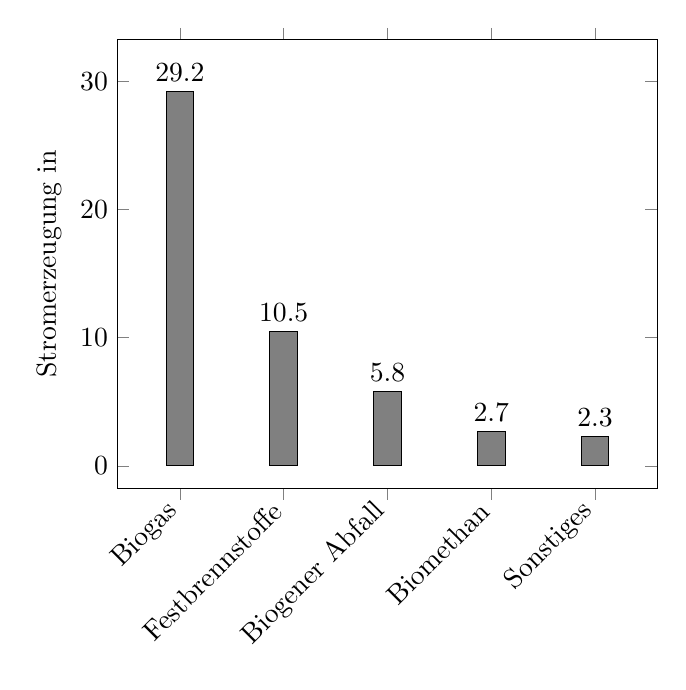
\begin{tikzpicture}
		\begin{axis}[
		ybar,
		enlargelimits=0.15,											% äüßerste bar plots nicht am Limit der x-Achse
		legend style={at={(0.5,-0.2)},
		anchor=north,legend columns=-1},
		ylabel={Stromerzeugung in \SI{}{\twh}},
		symbolic x coords={Biogas,
			Festbrennstoffe,
			Biogener Abfall,
			Biomethan,
			Sonstiges 
		},
		xtick=data,
		nodes near coords,											% Zahlen auf den bar plots
		nodes near coords align={vertical},
		x tick label style={rotate=45,anchor=east},
		]
		\addplot[black,fill=black!50!white] coordinates {
			(Biogas,29.2) (Festbrennstoffe,10.5) (Biogener Abfall,5.8)
			(Biomethan,2.7) (Sonstiges,2.3)
		};
		\end{axis}
	\end{tikzpicture}
	\caption{Verteilung der Bruttostromerzeugung aus Biomasse nach Erzeugungsart im Jahr 2019 \parencite{BWE2020}; Eigene Darstellung}
	\label{fig:ee-gen_biomass}
\end{figure}